% =====================================================================
% CC-ResDiff -- EACE-2026 submission version (target: 10 pages).
%
% This is the CONDENSED version. paper/cc_resdiff.tex remains the extended
% draft and is the reference for anything cut here.
%
% BEFORE SUBMITTING:
%  1. Replace this preamble with the official EACE / Springer LNEE template.
%     The conference requires .doc/.docx, so this file is the content source,
%     not the submission artefact.
%  2. Fill in affiliation and email (marked TODO below).
%  3. Verify every bibliography entry. They were drafted from memory; venues,
%     years and page numbers have NOT been checked against the actual papers.
%  4. Confirm with the organisers whether single- or double-spacing governs the
%     10-page count. It roughly halves what fits and changes how much to cut.
% =====================================================================
\documentclass[10pt]{article}
\usepackage[margin=1in]{geometry}
\usepackage{amsmath,amssymb}
\usepackage{booktabs}
\usepackage{graphicx}
\usepackage[hidelinks]{hyperref}
\newcommand{\best}[1]{\textbf{#1}}

\title{\textbf{CC-ResDiff: Bounding Seed-Dependent Color Drift in
Residual-Space Diffusion Super-Resolution}}
\author{Sudhir Kumar\\
\small TODO: Department, Institution, City, Country\\
\small \texttt{TODO: email@institution.edu}}
\date{}

\begin{document}
\maketitle

\begin{abstract}
Residual-space diffusion models for super-resolution, such as SRDiff and
ResDiff, train a diffusion model to predict the residual between a CNN
prediction and the ground truth. Because that residual is mostly
high-frequency, and recent work strengthens high-frequency guidance further,
the global color of the output is never supervised directly. ResDiff reports the
consequence---visible color discrepancy in under-trained models---and proposes a
global color feature as future work. We implement that proposal as a Global
Color-Consistency (GCC) loss: an auxiliary term comparing spatially pooled color
statistics of the model's implied clean prediction with the ground truth. It is
training-time only and leaves inference cost unchanged. Our main finding concerns the
baseline rather than the loss: across three seeds of an otherwise identical
configuration, baseline color error varies over $0.14$--$0.82$, so single-run
comparisons of color-consistency methods are unreliable.
Against that variability the GCC loss acts as a stabiliser, confining color error
to $0.15$--$0.26$ across five paired experimental configurations spanning two datasets and an $8\times$
range of training-set size, with $6.5\times$ lower standard deviation. It bounds color drift where it occurs rather than
improving color uniformly, recovering most of the gap on runs that drift and
remaining neutral on those that do not---which also explains a DIV2K result that
in isolation reads as a failure to generalise. The trade-off is explicit: PSNR, SSIM and
LPIPS are unchanged within seed noise, and FID is consistently worse by $2.73$.
We report that regression, and an ablation refuting our own explanation for it.
\end{abstract}

\noindent\textbf{Keywords:} image super-resolution, diffusion models, color
consistency, auxiliary loss, training stability, seed variance, residual
learning, generative models

\section{Introduction}

Single image super-resolution (SISR) is ill-posed. Adversarial
methods~\cite{ledig2017photo,wang2018esrgan} were long dominant but train
unstably; denoising diffusion models~\cite{ho2020denoising} have largely
displaced them. Residual-space variants are the strongest of these for SISR:
SRDiff~\cite{li2022srdiff} and ResDiff~\cite{shang2024resdiff} first use a CNN to
recover low-frequency content, then train a diffusion model to generate only the
\emph{residual} between that prediction and the ground truth, which accelerates
convergence.

This design has an under-examined consequence. The residual is mostly
high-frequency, and the $\epsilon$-prediction objective supervises the noise
added to it, so nothing constrains the absolute color of the reconstruction.
ResDiff sharpens the imbalance by adding frequency-domain losses and
high-frequency-guided cross-attention---improving detail while supplying no color
signal---and observes the result directly, noting that ``the color will appear a
large discrepancy when the model is under-trained,'' attributing it to ``a lack of
color features in the guided high-frequency information,'' and proposing that
``utilizing a global color feature may well address this issue in future
work''~\cite{shang2024resdiff}. We take up that proposal.

\paragraph{Contributions.}
(i) A Global Color-Consistency loss for residual-space diffusion SISR, adding no
parameters and leaving sampling unchanged, so inference cost is identical to the
baseline. (ii) The observation that \emph{baseline} color drift is itself strongly
seed-dependent, varying sixfold across identical configurations, which implies
single-run comparisons of color-consistency methods---including the first run of
our own---can misstate an effect severalfold. (iii) A gradient-level analysis
showing the auxiliary term's influence spans five orders of magnitude across the
diffusion trajectory, with an ablation identifying that skew as the mechanism
rather than an artefact. (iv) An explicit account of the costs: no distortion
benefit, and a consistent FID regression we could not explain.

\section{Related Work}

\paragraph{Diffusion SISR.}
SR3~\cite{saharia2022image} conditions DDPM on an upsampled LR image.
SRDiff~\cite{li2022srdiff} introduces residual prediction;
ResDiff~\cite{shang2024resdiff} adds frequency-domain guidance. The trajectory of
this line is towards stronger high-frequency supervision, leaving low-frequency
content to the CNN and never supervising it directly.

\paragraph{Color correction and loss weighting.}
Established color methods are corrective and act outside the model: per-channel
statistic matching~\cite{reinhard2001color}, full distribution
transfer~\cite{pitie2005ndim} and color
constancy~\cite{barron2015convolutional,afifi2019color} all require a reference or
an illuminant estimate at test time. Section~\ref{sec:ct} shows that distinction
is decisive rather than academic. Separately, timestep reweighting of the
\emph{primary} diffusion objective is well
studied~\cite{nichol2021improved,choi2022perception,hang2023efficient}; we show
that an \emph{auxiliary} loss on the reconstructed $x_0$ inherits an extreme
implicit weighting whether or not its designer intends it.

\section{Method}

Let $x_{LR}$, $x_{HR}$ and $x_{up}$ denote the LR input, the ground truth and the
bicubically upsampled input. Residual diffusion targets $r = s\,(x_{HR} - x_{up})$,
clipped to $[-1,1]$, with the usual forward process
$r_t = \sqrt{\bar\alpha_t}\,r + \sqrt{1-\bar\alpha_t}\,\epsilon$ and objective
\begin{equation}
\mathcal{L}_{\text{DDPM}} = \mathbb{E}\big[\|\epsilon - \epsilon_\theta(r_t,t,c)\|_1\big],
\label{eq:ddpm}
\end{equation}
where $c$ is CNN-derived conditioning. Nothing in Eq.~\ref{eq:ddpm} references the
absolute color of the reconstruction.

We recover the implied clean residual through the standard closed form,
\begin{equation}
\hat r_0 = \frac{r_t - \sqrt{1-\bar\alpha_t}\,\epsilon_\theta(r_t,t,c)}{\sqrt{\bar\alpha_t}},
\label{eq:x0}
\end{equation}
clamp it to $[-1,1]$, map it back to image space as $\hat x_{HR} = \hat r_0/s + x_{up}$,
and compare pooled color statistics:
\begin{equation}
\mathcal{L}_{\text{GCC}} = \big\|\mathcal{P}_k(\hat x_{HR}) - \mathcal{P}_k(x_{HR})\big\|_2^2 ,
\label{eq:gcc}
\end{equation}
and add it to the primary objective with a single weight $\lambda$:
\begin{equation}
\mathcal{L} = \mathcal{L}_{\text{DDPM}} + \lambda\,\mathcal{L}_{\text{GCC}} .
\label{eq:total}
\end{equation}
with $\mathcal{P}_k$ adaptive average pooling to a $k \times k$ grid. Pooling is
what makes Eq.~\ref{eq:gcc} complementary rather than redundant:
texture and edges, retaining only the spatial color balance that
Eq.~\ref{eq:ddpm} leaves unconstrained.

Eq.~\ref{eq:total} is the complete objective; the remainder of the training
step is unchanged. Two implementation details are load-bearing. Eq.~\ref{eq:x0} must be evaluated in
fp32: under a cosine schedule $\bar\alpha_t$ reaches $2.4\times10^{-7}$ at
$t = T-1$, so the reconstruction amplifies by ${\sim}2000\times$ and overflows
fp16 under mixed precision. And the clamp cannot be omitted---unclamped we
measured $\mathcal{L}_{\text{GCC}} = 2.8\times10^{4}$ at $t = T-1$ against a DDPM
loss of ${\sim}0.8$, so with $t$ sampled uniformly roughly one step in a hundred
would destabilise training. Sampling is untouched, so inference cost equals the
baseline's.

\section{Experiments}

\paragraph{Setup.}
CelebA~\cite{liu2015faceattributes} subsampled to 3{,}000 training and 300 test
images at $16\times16 \to 64\times64$ ($4\times$). Stage 1 is an RRDB; Stage 2 a
$2.28$M-parameter UNet, $T=100$, cosine schedule, up to 20{,}000 steps with early
stopping on PSNR. The two arms are identical in data, schedule, seed,
initialisation and Stage-1 checkpoint, differing only in the GCC term. Early
stopping monitors PSNR rather than color error, so model selection cannot favour
the proposed arm.

\paragraph{Scope.}
Our baseline is SRDiff. ResDiff motivates this work but is not
reimplemented---its FD Info Splitter, HF-guided cross-attention and FFT/DWT losses
are absent here---so every comparison is SRDiff versus SRDiff plus GCC. Absolute
values are therefore not comparable with published SRDiff, ResDiff or SR3
results, which use different tasks ($64\to256$, $20\to160$, $40\to160$), full
training sets and larger models; our FID is computed over 300 images, which biases
it upward. We make no state-of-the-art claim.

\paragraph{Metrics.}
PSNR, SSIM~\cite{wang2004image}, LPIPS~\cite{zhang2018unreasonable} and
FID~\cite{heusel2017gans}, plus \emph{color error}: the mean absolute difference
between per-channel RGB means of the output and the ground truth, in $0$--$255$
units. We also report LR-PSNR, which measures low-frequency fidelity and is thus
the quantity GCC most directly targets. Evaluating one fixed checkpoint under four
seeds gives an evaluation noise floor (std): PSNR $0.018$, SSIM $0.0004$, LPIPS
$0.0005$, LR-PSNR $0.009$, color error $0.0022$, FID $0.15$.

\subsection{Baseline Color Drift is Seed-Dependent}
\label{sec:main}

Table~\ref{tab:perrun} is the paper's central result, and it concerns the
baseline. Under configurations differing only in random seed, baseline color error
ranges from $0.14$ to $0.82$---a sixfold spread, orders of magnitude beyond the
$0.0022$ evaluation noise floor. Under the evaluated configuration, whether substantial color drift
occurs is therefore strongly influenced by the random training seed.

This carries a methodological consequence independent of our loss: a single-run
comparison of any color-consistency method can overstate or understate its effect
severalfold. Our own first run showed a $-70.6\%$ reduction and our third a
$+4.6\%$ increase; reporting either alone would have been misleading.

\begin{table}[t]
\centering\small
\begin{tabular}{lccc}
\toprule
Run & Baseline & CC-ResDiff & Change \\
\midrule
CelebA 3k, seed A   & 0.8234 & 0.2423 & $-70.6\%$ \\
CelebA 3k, seed B   & 0.3878 & 0.2061 & $-46.9\%$ \\
CelebA 3k, seed C   & 0.1397 & 0.1461 & $+4.6\%$ \\
CelebA 25k          & 0.2948 & 0.2555 & $-13.3\%$ \\
DIV2K               & 0.1650 & 0.2036 & $+23.4\%$ \\
\midrule
\emph{std across runs} & \emph{0.2767} & \emph{0.0426} & \\
\emph{range}           & \emph{0.684}  & \emph{0.109}  & \\
\bottomrule
\end{tabular}
\caption{Color error across five paired experimental configurations spanning two datasets and an
$8\times$ range of training-set size. The baseline spans $0.14$--$0.82$;
CC-ResDiff stays within $0.15$--$0.26$.}
\label{tab:perrun}
\end{table}

Against that variability the GCC loss acts as a stabiliser: its color error falls
within $0.15$--$0.26$ in every configuration, with a $6.5\times$ smaller standard deviation
and a $6.2\times$ narrower range. We describe this as \emph{bounding} color drift
rather than reducing it, and are deliberate about the strength of the claim: the three-seed CelebA experiment is the only
replicated evidence here---the 25k and DIV2K tiers are single runs---so these five
configurations establish a consistent stabilising effect in our experiments
rather than a formal guarantee. The benefit on any given run is governed by how far its baseline
sits outside CC-ResDiff's band, which is why one mechanism produces both the
$-70.6\%$ run and the DIV2K increase.

We deliberately omit one tempting statistic. The correlation between a run's
baseline color error and the improvement obtained is $r = 0.997$, but improvement
is defined as $c_{\text{CC}} - c_{\text{base}}$, so the baseline appears on both
sides and the correlation is mechanically induced---it would be near unity even
for random output. The variance comparison in Table~\ref{tab:perrun} carries the
same content without that coupling.

\subsection{Aggregate Results and the FID Trade-off}

Table~\ref{tab:main} reports all metrics over three CelebA seeds. Only color error
and FID differ by more than their across-seed spread. In particular, the
$-0.13$\,dB PSNR cost visible in our first run did not replicate: at $n=3$ the mean
is $-0.002$\,dB, and the apparent cost was seed noise.

\begin{table}[t]
\centering\small
\begin{tabular}{lccc}
\toprule
Metric & Baseline & CC-ResDiff & $\Delta$ \\
\midrule
Color error $\downarrow$ & $0.4494 \pm 0.3446$ & \best{$0.1981 \pm 0.0486$} & $-0.2512$ \\
LR-PSNR $\uparrow$       & $44.66 \pm 0.82$ & \best{$44.95 \pm 0.66$} & $+0.29$ \\
PSNR $\uparrow$          & \best{$25.033 \pm 0.082$} & $25.031 \pm 0.075$ & $-0.002$ \\
SSIM $\uparrow$          & \best{$0.8143 \pm 0.0022$} & $0.8141 \pm 0.0021$ & $-0.0002$ \\
LPIPS $\downarrow$       & \best{$0.0439 \pm 0.0020$} & $0.0446 \pm 0.0021$ & $+0.0007$ \\
FID $\downarrow$         & \best{$66.70 \pm 2.19$} & $69.43 \pm 3.59$ & $+2.73$ \\
\bottomrule
\end{tabular}
\caption{CelebA $4\times$, mean $\pm$ std over three training runs. Note the
standard deviations: the baseline's color error varies by an order of magnitude
more than CC-ResDiff's.}
\label{tab:main}
\end{table}

\textbf{The FID regression is the method's principal cost, and we state it
plainly.} FID is worse in all four CelebA configurations tested---three seeds plus
the larger-data tier---by $+2.73$ on average. Section~\ref{sec:grad} reports an
experiment that refutes our own explanation for it, so the cause remains open. A
practitioner should adopt GCC as a targeted mechanism for controlling
seed-dependent color drift, not as a general improvement to perceptual quality.

\begin{figure}[htbp]
\centering
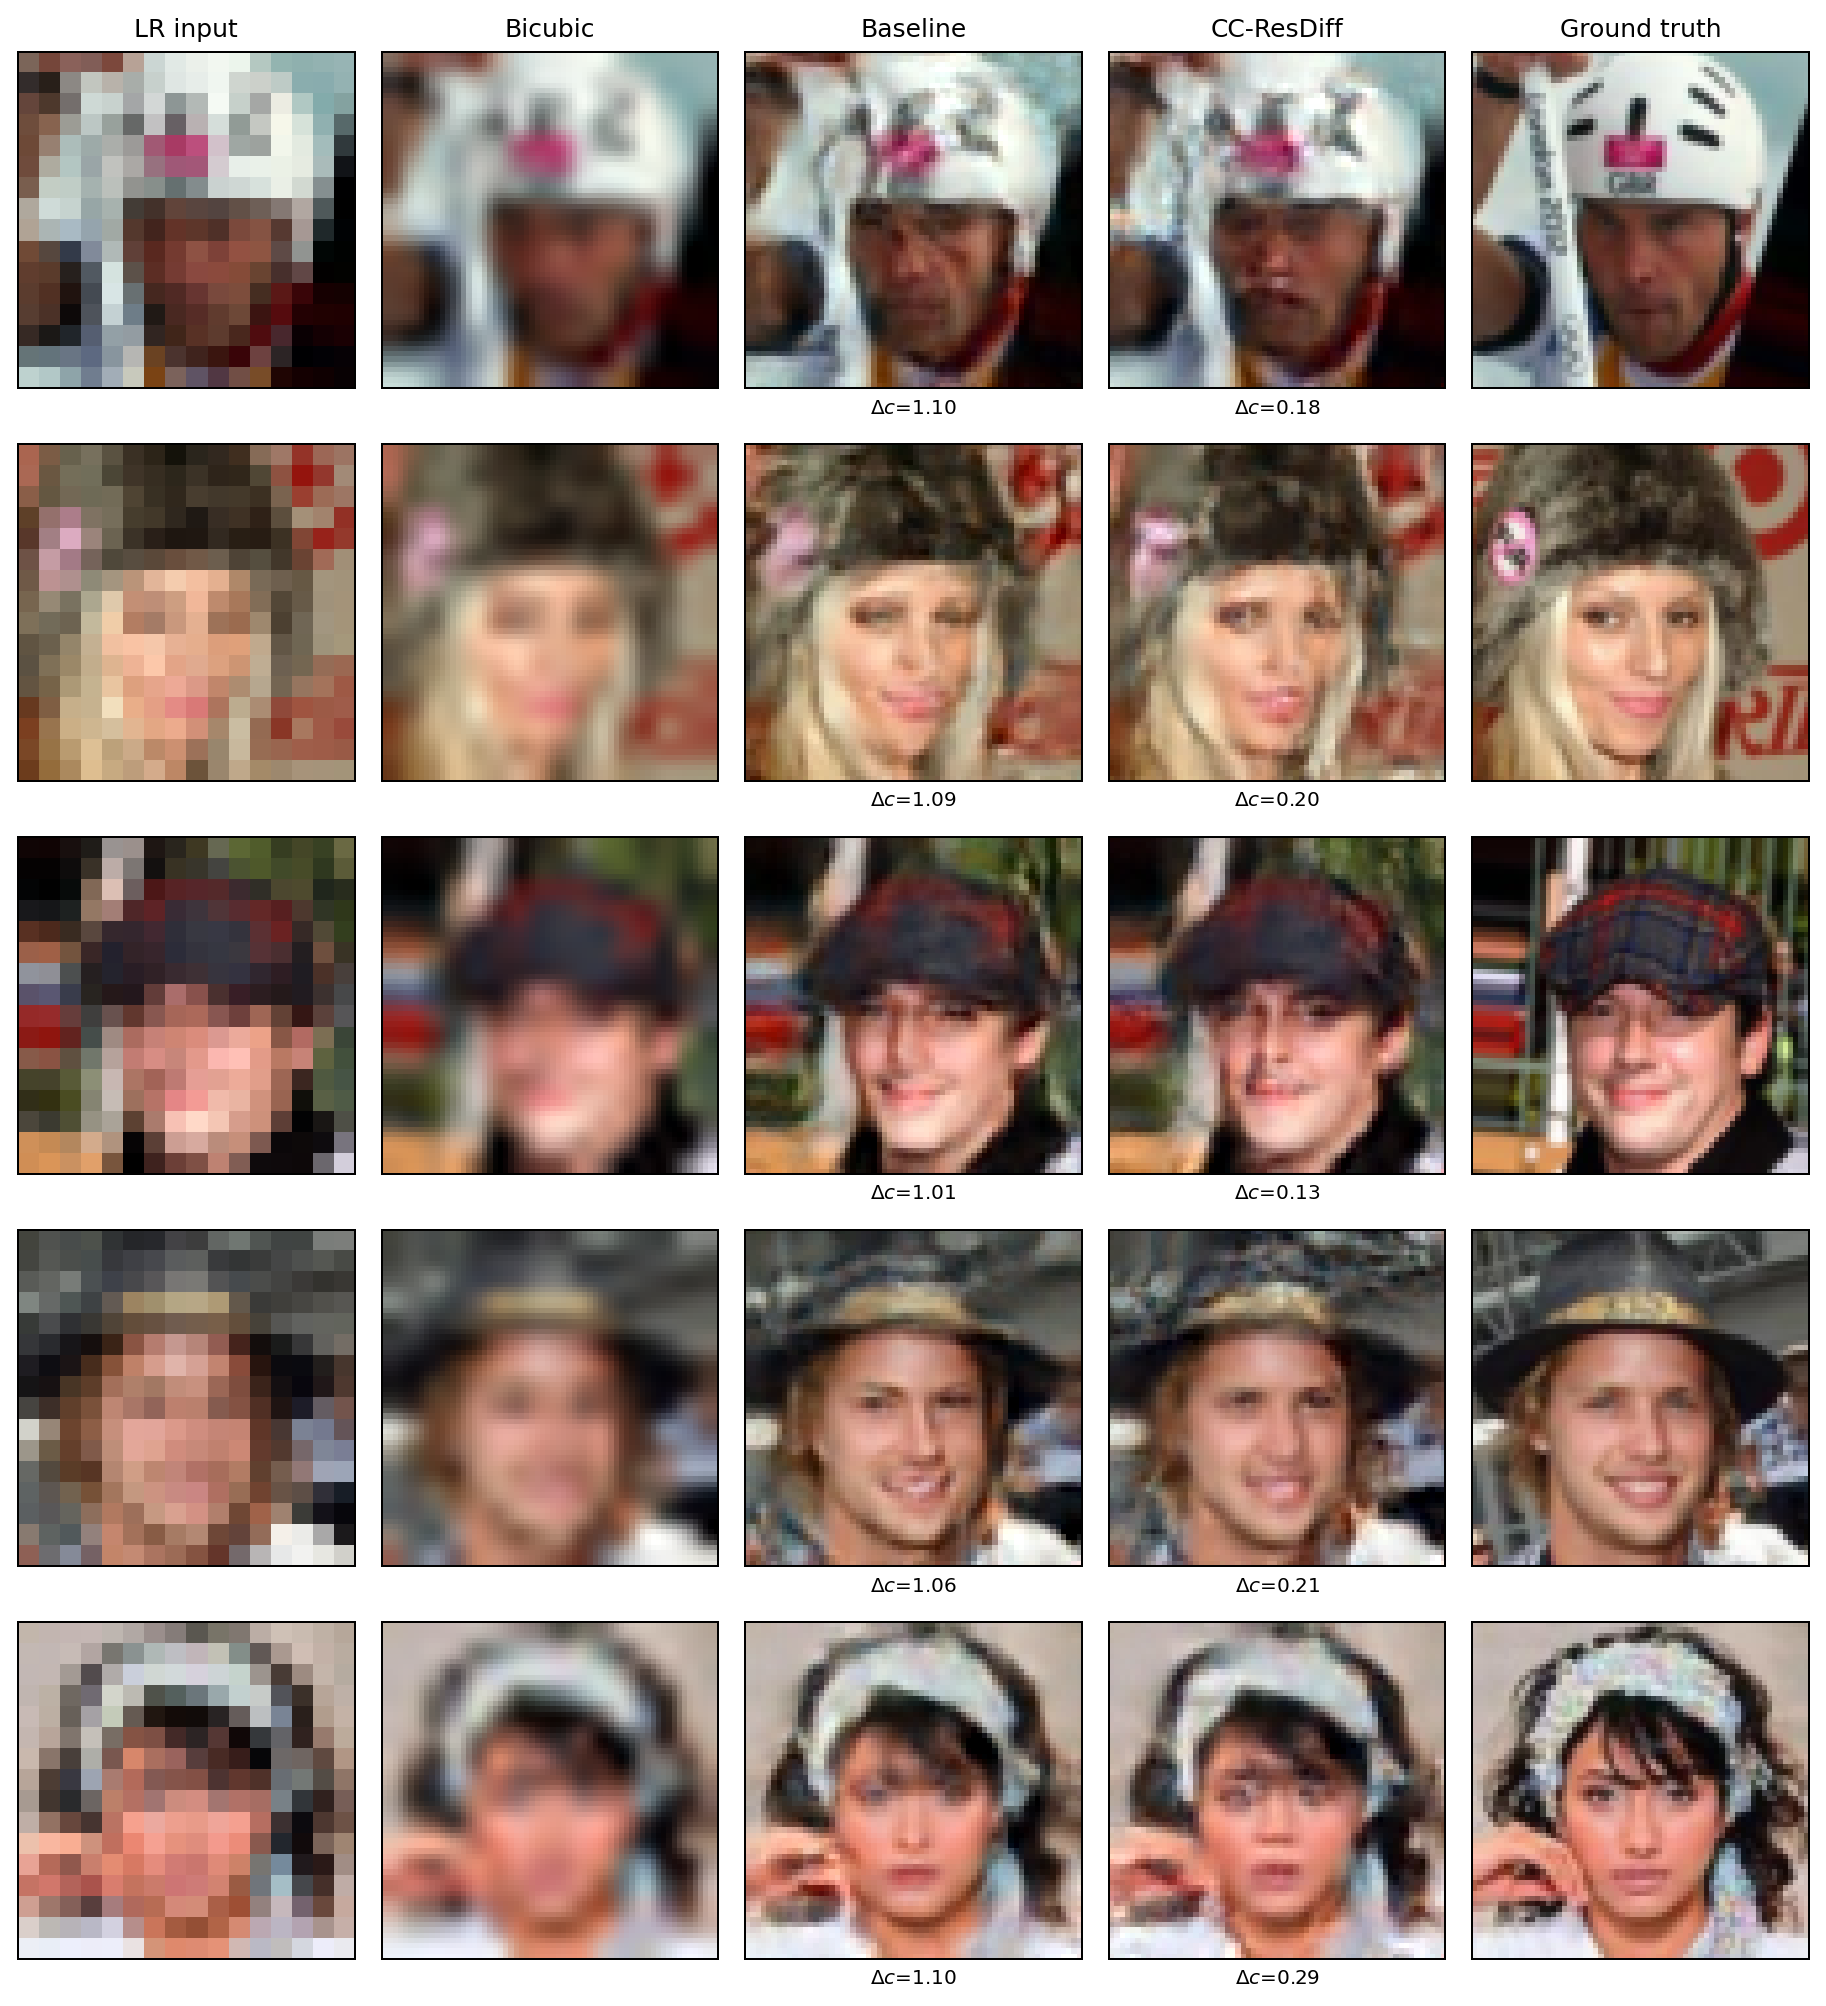
\includegraphics[width=0.82\linewidth]{qualitative.png}
\caption{CelebA $4\times$: LR input, bicubic, baseline, CC-ResDiff, ground truth.
Rows are the test images with the largest color-error difference, a selection rule
chosen to display the phenomenon under discussion; per-image color error
$\Delta c$ is printed beneath each result. Differences are measurable but visually
subtle: color error is in $0$--$255$ units, so $0.82 \to 0.24$ is a sub-one-level
shift---far above the $0.0022$ measurement noise and consistent across $298/300$
images, yet near the limit of perceptibility.}
\label{fig:qual}
\end{figure}

\subsection{Post-hoc Color Correction is Insufficient}
\label{sec:ct}

A natural objection is that cheap post-processing might achieve the same effect.
We applied per-channel mean and mean/standard-deviation matching to the baseline's
outputs, using the upsampled LR image as reference---the only reference admissible
at inference, since matching to the ground truth would be unusable in practice.
Neither variant helps (Table~\ref{tab:ct}): both increase color error, and
matching the variance costs $7.4$\,dB of LR-PSNR by altering exactly the
low-frequency content LR-PSNR measures.

\begin{table}[t]
\centering\small
\begin{tabular}{lcc}
\toprule
Method & Color error $\downarrow$ & LR-PSNR $\uparrow$ \\
\midrule
Baseline                & 0.8234 & 43.690 \\
\quad + mean transfer      & 0.8746 & 43.558 \\
\quad + mean/std transfer  & 0.9333 & 36.243 \\
\emph{reference floor} ($x_{up}$ vs $x_{HR}$) & \emph{0.4358} & --- \\
CC-ResDiff              & \best{0.2423} & \best{44.509} \\
\bottomrule
\end{tabular}
\caption{Post-hoc color correction versus learned supervision, CelebA, 300 test
images.}
\label{tab:ct}
\end{table}

The reason is structural. Any post-hoc correction is bounded below by the accuracy
of the reference it matches to, and the upsampled LR image itself differs from the
ground truth by $0.4358$. CC-ResDiff reaches $0.2423$, below that floor, because
supervision is applied during training against the true HR image and no test-time
reference is required.

\subsection{Gradient Analysis and a Refuted Hypothesis}
\label{sec:grad}

Loss values suggest the GCC term is negligible---$0.06\%$ of the DDPM loss at
$\lambda = 0.1$. Its \emph{gradient} tells a different story
(Table~\ref{tab:grad}): $33.9\%$ of the DDPM gradient averaged over uniformly
sampled $t$, some $500\times$ more than the loss ratio implies, and spanning five
orders of magnitude across the trajectory. The clamp bounds the loss value but not
the gradient: at $t = T-1$ nearly all elements saturate, yet the remainder still
carry the ${\sim}2000\times$ amplification.

\begin{table}[t]
\centering\small
\begin{tabular}{lccc}
\toprule
$t$ & $0$ & $75$ & $T-1$ \\
\midrule
Clamped fraction & $0.4\%$ & $0.1\%$ & $97.4\%$ \\
Gradient ratio to $\mathcal{L}_{\text{DDPM}}$ & $0.002\%$ & $1.28\%$ & \best{$235.7\%$} \\
\midrule
\multicolumn{4}{l}{\emph{Over uniformly sampled $t$: $33.9\%$}} \\
\bottomrule
\end{tabular}
\caption{The GCC term's gradient contribution is concentrated at large $t$,
spanning five orders of magnitude.}
\label{tab:grad}
\end{table}

This suggested a hypothesis: if the term acts predominantly at large $t$, and that
is what pulls global tone toward the dataset mean, then cancelling the skew by
weighting with $w_t = \bar\alpha_t$ should remove the FID regression while
retaining the color benefit. The reweighting is effective as an intervention,
taking the $t = T-1$ versus $t = 0$ gradient ratio from $2029\times$ down to
$0.0005\times$. The hypothesis, however, is wrong. FID becomes \emph{worse}
($77.81$ versus $73.23$), the color benefit largely disappears ($0.673$ versus
$0.242$), and the LR-PSNR gain vanishes entirely; the reweighted variant loses on
every metric we measure.

Two conclusions follow. The concentration at large $t$ is the \emph{mechanism},
not a defect: large-$t$ steps determine global low-frequency structure while
small-$t$ steps refine local detail, so a global color loss should act at large
$t$, and an implementation that spread it uniformly would supervise color where
color is no longer being decided. And the cause of the FID regression remains
unexplained---we report the refutation rather than leave an untested explanation
in the literature. More generally, any auxiliary loss defined on the reconstructed
$x_0$ inherits this implicit weighting; we recommend reporting gradient ratios
rather than loss ratios whenever such a term is introduced.

\subsection{Ablations, Scale, and When the Loss Helps}

At a reduced 5{,}000-step budget, with an identical budget for every run so the
sweep does not partly measure training length (Table~\ref{tab:abl}), pool size
$k=8$ is best on every metric and five of six GCC settings beat the no-GCC
reference on color error. LPIPS degrades monotonically in $\lambda$ and FID
worsens past $\lambda = 0.01$, so the cost side is consistent. We do \emph{not}
claim an optimal $\lambda$: color error across the six settings has standard
deviation $0.109$, comparable to the differences between them, so the sweep
supports a usable range ($\lambda \in [0.01, 0.1]$, $k = 8$) rather than a
dose-response curve.

\begin{table}[t]
\centering\small
\begin{tabular}{lcccc}
\toprule
Setting & Color err. $\downarrow$ & PSNR $\uparrow$ & LPIPS $\downarrow$ & FID $\downarrow$ \\
\midrule
no GCC           & 0.4833 & 23.857 & \best{0.0612} & 111.51 \\
$\lambda = 0.01$ & 0.3382 & \best{23.955} & 0.0635 & \best{109.11} \\
$\lambda = 0.1$  & \best{0.1952} & 23.941 & 0.0653 & 110.43 \\
$\lambda = 0.5$  & 0.4985 & 23.721 & 0.0665 & 115.43 \\
$\lambda = 1.0$  & 0.2162 & 23.727 & 0.0680 & 116.71 \\
\midrule
$k = 4$          & 0.3385 & 23.839 & 0.0641 & 112.47 \\
$k = 16$         & 0.3522 & 23.919 & 0.0658 & 111.05 \\
\bottomrule
\end{tabular}
\caption{Ablations at a 5{,}000-step budget; pool $k=8$ unless stated, and
$\lambda = 0.1$ for the $k$ rows. These runs are comparable to each other, never
to Table~\ref{tab:main}.}
\label{tab:abl}
\end{table}

\paragraph{Scale.}
Repeating the experiment with $8\times$ the data (25{,}000 images) and Stage 1 at
full capacity, on an identical test split, improves absolute quality
substantially: PSNR $25.03 \to 25.43$, LR-PSNR $44.66 \to 47.63$, FID
$66.70 \to 61.83$. The GCC benefit falls to $-13.3\%$, but only because the
baseline now drifts less ($0.4494 \to 0.2948$); CC-ResDiff's own color error
($0.2555$) stays inside its usual band. This is a fifth confirmation of the
bounding behaviour, obtained under conditions chosen to break it.

\paragraph{DIV2K.}
At matched scale on DIV2K~\cite{agustsson2017ntire}, color error rises from
$0.1650$ to $0.2036$ and every other sign flips relative to CelebA. Read against
Section~\ref{sec:main} this is not a separate phenomenon: DIV2K's baseline sits in
the low-drift band alongside CelebA seed C ($0.1397$), so there is nothing to
recover, and CC-ResDiff's own value again lands in its usual range. Per tile,
CC-ResDiff has lower color error on $171/512$ DIV2K tiles ($33.4\%$) against
$298/300$ CelebA images ($99.3\%$); on DIV2K the two arms are visually indistinguishable.
Figure~\ref{fig:qual} shows CelebA examples, where the effect is present.

\section{Limitations}

Our experiments use 3{,}000 CelebA images at $64\times64$ with a $2.28$M-parameter
diffusion model, and 25{,}000 at the larger tier---far below the resolutions and
model sizes used by SRDiff and ResDiff, so whether the effect persists there is
untested. We have three seeds on the main CelebA tier and one run each on the 25k
and DIV2K tiers: enough to establish that baseline drift varies widely while
CC-ResDiff's does not, but not to characterise either distribution or to place a
confidence interval on the bound. We have no DIV2K noise floor, so the $+23.4\%$
there is not established as statistically real. FID over 300 images is biased
upward and meaningful only as a relative comparison on identical images, and
DIV2K metrics cover image interiors because partial edge tiles are dropped at
packing time. The effect size is small in absolute terms---a sub-one-level shift
in mean channel intensity---and we cannot predict in advance which training
configurations will drift.

\section{Conclusion}

We implemented the global color feature that ResDiff identified as future work
and, in characterising it, arrived at a different claim than we set out to make.
The reliable finding is that \emph{baseline} color drift in residual diffusion
SISR is strongly seed-dependent, varying sixfold across identical
configurations---which makes single-run comparisons of color-consistency methods
unreliable, our own first run included. Against that variability the GCC loss is a
stabiliser: it confines color error to a narrow band in every run we performed, on
both datasets and at both data scales, at no parameter or inference cost. What it
buys is predictability rather than average improvement, and it costs a consistent
FID regression that we report and could not explain. Two results were not what we
expected: the implicit timestep weighting an auxiliary $x_0$ loss inherits proved
to be the source of the benefit rather than a flaw, and our mechanism-based
account of the FID regression was falsified by the same ablation. Establishing
confidence intervals on the bound, and predicting which configurations drift, are
the natural next steps.

\begin{thebibliography}{99}
\small
% VERIFY EVERY ENTRY -- drafted from memory; venues, years and pages unchecked.
\bibitem{shang2024resdiff} S.~Shang et al. ResDiff: Combining CNN and Diffusion Model for Image Super-Resolution. {\em AAAI}, 2024.
\bibitem{li2022srdiff} H.~Li et al. SRDiff: Single Image Super-Resolution with Diffusion Probabilistic Models. {\em Neurocomputing}, 479:47--59, 2022.
\bibitem{saharia2022image} C.~Saharia et al. Image Super-Resolution via Iterative Refinement. {\em IEEE TPAMI}, 2023.
\bibitem{ho2020denoising} J.~Ho, A.~Jain and P.~Abbeel. Denoising Diffusion Probabilistic Models. {\em NeurIPS}, 2020.
\bibitem{nichol2021improved} A.~Nichol and P.~Dhariwal. Improved Denoising Diffusion Probabilistic Models. {\em ICML}, 2021.
\bibitem{choi2022perception} J.~Choi et al. Perception Prioritized Training of Diffusion Models. {\em CVPR}, 2022.
\bibitem{hang2023efficient} T.~Hang et al. Efficient Diffusion Training via Min-SNR Weighting Strategy. {\em ICCV}, 2023.
\bibitem{ledig2017photo} C.~Ledig et al. Photo-Realistic Single Image Super-Resolution Using a Generative Adversarial Network. {\em CVPR}, 2017.
\bibitem{wang2018esrgan} X.~Wang et al. ESRGAN: Enhanced Super-Resolution Generative Adversarial Networks. {\em ECCV Workshops}, 2018.
\bibitem{reinhard2001color} E.~Reinhard et al. Color Transfer between Images. {\em IEEE Computer Graphics and Applications}, 21(5):34--41, 2001.
\bibitem{pitie2005ndim} F.~Piti\'e et al. N-Dimensional Probability Density Function Transfer and its Application to Colour Transfer. {\em ICCV}, 2005.
\bibitem{barron2015convolutional} J.~T.~Barron. Convolutional Color Constancy. {\em ICCV}, 2015.
\bibitem{afifi2019color} M.~Afifi et al. When Color Constancy Goes Wrong: Correcting Improperly White-Balanced Images. {\em CVPR}, 2019.
\bibitem{heusel2017gans} M.~Heusel et al. GANs Trained by a Two Time-Scale Update Rule Converge to a Local Nash Equilibrium. {\em NeurIPS}, 2017.
\bibitem{zhang2018unreasonable} R.~Zhang et al. The Unreasonable Effectiveness of Deep Features as a Perceptual Metric. {\em CVPR}, 2018.
\bibitem{wang2004image} Z.~Wang et al. Image Quality Assessment: From Error Visibility to Structural Similarity. {\em IEEE TIP}, 13(4):600--612, 2004.
\bibitem{liu2015faceattributes} Z.~Liu et al. Deep Learning Face Attributes in the Wild. {\em ICCV}, 2015.
\bibitem{agustsson2017ntire} E.~Agustsson and R.~Timofte. NTIRE 2017 Challenge on Single Image Super-Resolution: Dataset and Study. {\em CVPR Workshops}, 2017.
\end{thebibliography}

\end{document}
